\chapter{Experiment and Evaluation}

\section{Experimental Settings}
This section describes the general experimental settings applied to all the following experiments, for different experiments, their additional settings will be described in corresponding sections. For the fairness, all the evaluation are eventually conducted on the pre-processed ``raw'' data without any futher transformation. This decision is made because of the facts: (1)
different represent methods generate varying number of features, and the number of features will affect the computation of indexes listed in Section~\ref{sec:metrics}; (2) the separation quality could be good on the transformed data, but may not also acceptable on the original data, in term of the trend analysis, the latter one is more important. 

\subsection{The choice of group centers}
The generated groups could be mess, and it is necessary to highlight their centers when analyse their trends. In addition, some indexes requires knowing the cluster centers. One simplest way to extract the representative in a group is computing the arithmetic mean of that group. This method is called Euclidean Barycenter, it minimize the summed euclidean distance of that group. However, this method could be inappropriate when the original data are not aligned well. This is illustrated in Figure~\ref{fig:barycenter1}, where the red lines represent the computed centers and black lines represent the data points in the group. To better reveal the general trend of a group, the Dynamic Time Warping (DTW) based methods are used to compute the barycenter. As mentioned before, DTW is a distance measure that can be used to compare two un-aligned sequences. Since it uses the dynamic programming, its time complexity is $O(mn)$, where $m$ and $n$ are the length of that two sequences respectively. To reduce the time complexity, one of its variation ``Soft-DTW'' is used to compute the center. The computation details of Soft-DTW can be found in \cite{schultz2018nonsmooth}. The second row of the figure shows the center computed by Soft-DTW with $\gamma$ set to 1, compared with the Euclidean barycenter, this center is visually more representative. 
\begin{figure}[!htbp]
    \centering
    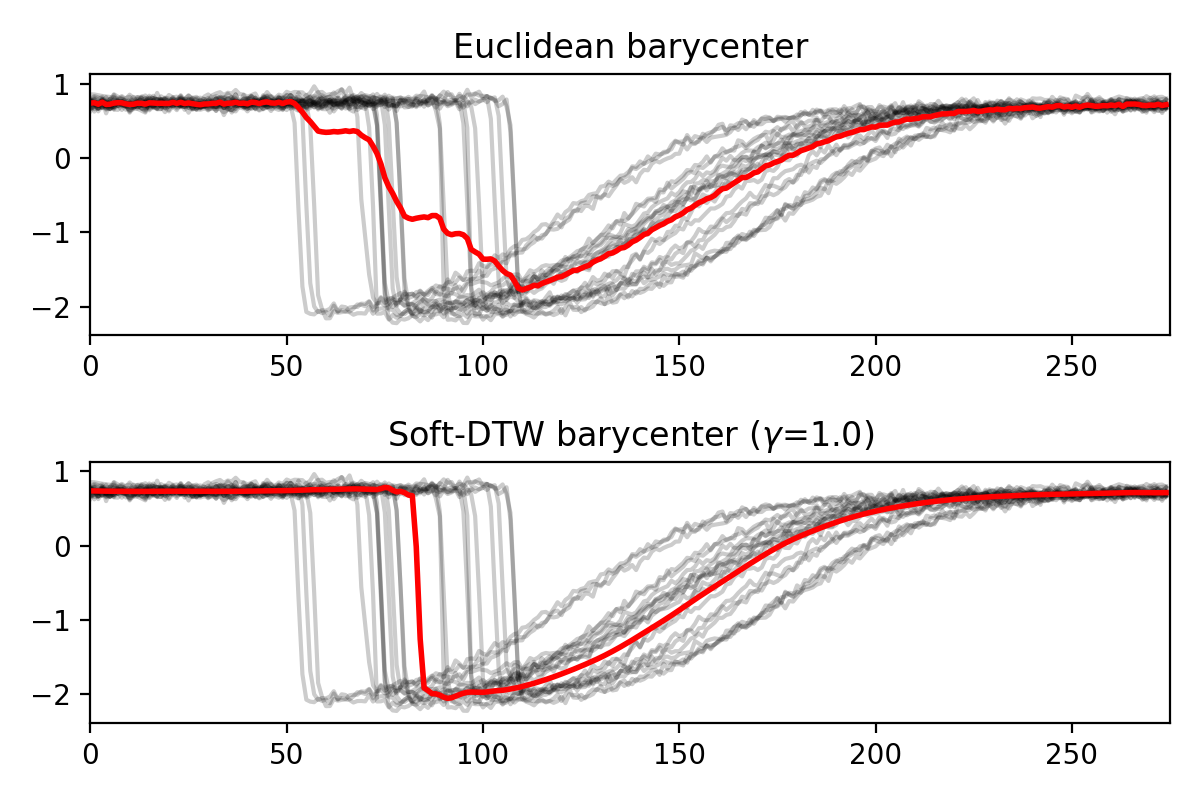
\includegraphics[width=0.6\columnwidth]{barycenter.png}
    \caption{Barycenter}
    \label{fig:barycenter1}
\end{figure} 

\subsection{Numerical Metrics}
\label{sec:metrics}
Generally, there are two indexes to evaluate the quality of data groups. The first one is the external index, it requires additional ground truth information to compare the generated groups with a reference model. The stock market dataset dose not contain such information, and hence the metric used here is the \textbf{internal index}. Literally, internal indexes reveal the intrinsic attributes of the groups, and does not require reference model. Within-cluster-scatter (WCS) and Between-cluster-scatter (BCS) are two basic internal indexes. The former one is introduced in Section~\ref{sec:reformulation}, it is the objective function of K-means algorithm, and it measures the compactness of clusters. Again, given a partition of $k (k>1)$ clusters $\Pi$, its equation is defined as:
\begin{equation}
    WCS(\Pi) = \sum_{i=1}^k \sum_{s=1}^{s_i} d^2(x_s^{(i)},m_i)
\end{equation}
Where $m_i$ denotes the center of cluster $i$, and $d(.,.)$ is distance measure.
\\\\To the contrary, BCS measures whether the clusters are well-separated, its equation is defined as:
\begin{equation}
    BCS(\Pi) = \sum_{i=1}^k s_i d^2(m,m_i)
    \label{eq:bcs}
\end{equation}
Where $s_i$ denotes the number of data points of cluster $i$ and $m$ denotes the center of all data points.
\\\\Intuitively, a good partition should get less WCS and higher BCS scores such that the clusters are more discriminative. This standard is used in this project since it is appropriate for stock market data analysis -- investors expect the trends being universal and distinguishable without any other information except the price sequences. 
\\\\To make the comparison more clear, an additional index is introduced. F-ratio index combines the WCS and BCS together, its equation is defined as:
\begin{equation}
    F(\Pi) = \frac{k WCS(\Pi)}{BCS(\Pi)} = \frac{k\sum_{i=1}^k \sum_{s=1}^{s_i} d^2(x_s^{(i)},m_i)}{\sum_{i=1}^k s_i d^2(m,m_i)}
    \label{eq:fratio}
\end{equation}
Lower F-ratio means better partitions. It's worth mentioning that DTW is selected as the distance measure and used to compute the centers of cluster. This decision is made to guarantee the local scaling invariance mentioned in the guideline. Figure~\ref{fig:dtwcode} shows the pseudocode of DTW.
\begin{figure}[!htbp]
    \centering
    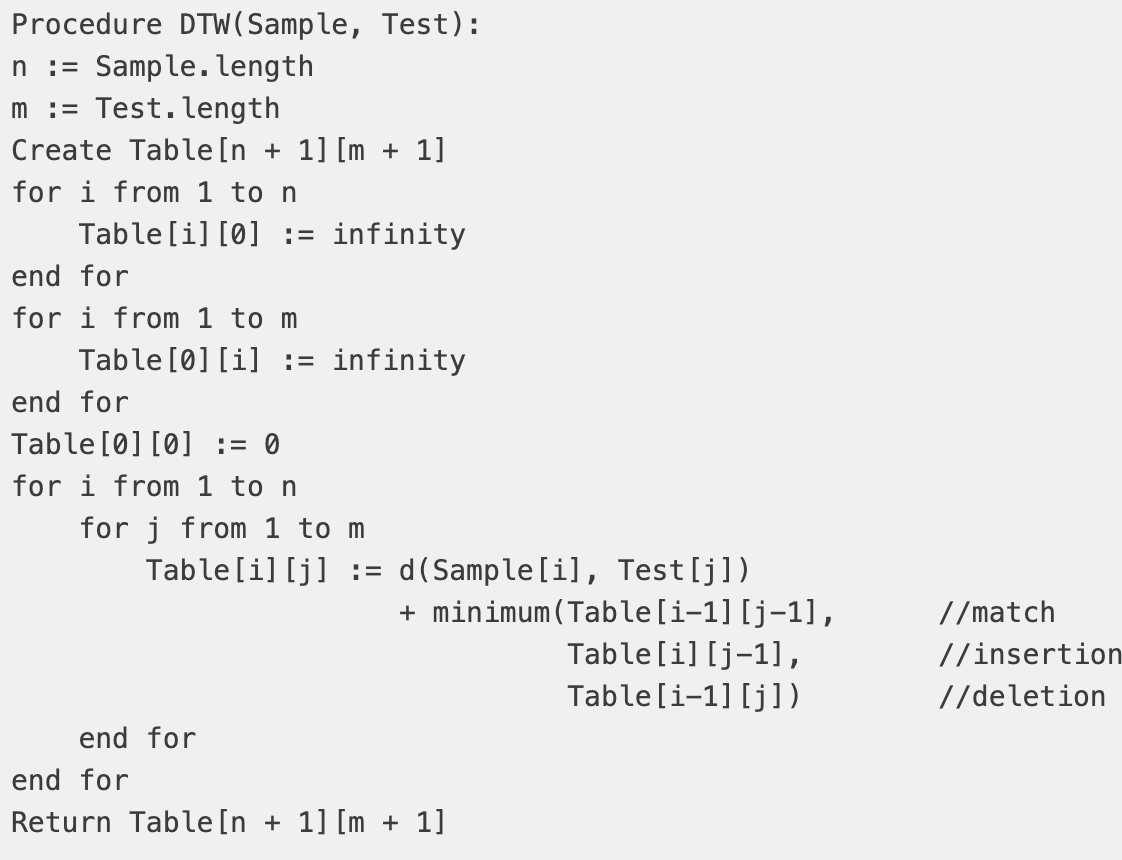
\includegraphics[width=0.6 \columnwidth]{dtw.png}
    \caption{Pseudocode of DTW}
    \label{fig:dtwcode}
\end{figure} 
\\\\There are other internal indexes such as the Silhouette Coefficient \cite{rousseeuw1987silhouettes} and Calinski-Harabasz index \cite{calinski1974dendrite}, but they indeed share the same objective with F-ratio but with slightly different formula, and hence they are not used as the metrics in this project.


\subsection{Main clustering algorithm}
The main clustering algorithm chosen to compare different representations is K-means. As mentioned before, its objective function is the WCS. To get the best partitions, traditional K-means adpots a greedy strategy, it works by: (1) first randomly initialise k cluster centers; (2) assign each data point to a cluster according to the distance measure; (3) updating the cluster centers with the mathematical mean of the data points in each cluster; (4) repeat step 2 and 3 until the stopping criteria are reached. 



\section{Comparison of PIP, PAA and Down Sampling}
In Section~\ref{sec:pippaa}, different similarity measures with visually similar stocks are used to evaluate the perfomance of three different sequence compression methods, and find that these three methods show no significant difference in terms of such measurement. However, as mentioned before, some compression methods can preserve key points while others can not, we believe this functionality does affect the final perfomance of some applications.  Therefore, this section is added to evaluate and verify the effectiveness of these three compression algorithms in the context of time series clustering task. The test data used here are the records of all stocks in our dataset. The number of clusters is limited up to 15 to tradeoff of the ease of visualization and the fairness of comparison.\\
\\For all these three methods, one parameter required is the compression ratio or the sequence length $c$. As mentioned before, there is no standard criterion to numerically evaluate the effect of compression ratio. The choice of sequence length $c$ depends highly on the given task, and it mostly done by trail and error. Here the most appropriate $c$ is chosen by using KMeans algorithms with the three indexes listed above. Figure~\ref{fig:comparison1} shows the experimental results. In all sub-figures, the three columns represent the SC score CH score and DB score respectively, while the blue, orange, green, red lines represent the scores of original version , PIP-compressed version, PAA-compressed version and down sampled version respectively. Again, higher SC and CH indicate better separation result, while higher DB means bad result. All 5 years data are used in the experiments, and the results are quite similar: \textbf{(1) using data compression algorithms does not improve the perfomance of KMeans algorithm with respect to the indexes used here; (2) Down Sampling gets the highest average score in all experiments with respect to the indexes used here;} (3) when $c$ is small (less than 50), PIP approache gets the worst perfomance with respect to the indexes used here; (4) when $c$ is large, PAA approache gets the worst perfomance with respect to the indexes used here; (5) within the given range, change $c$ does not significantly affect the final scores of Down Sampling; (6) the best ``c'' locates in range [50,70] for all approaches. To exclude the effect of algorithm itself, other clustering algorithms such agglomerative clustering algorithm are used, and get the similar observation. Observation (1) and (2) are against our assumptions, experimental results prove that down sampling indeed preserve the most shape information of the original sequence. Another interesting observations is that, in all 5 years, the best number of clusters is 2, and the overall score decreases when the number of cluster increases. 
\begin{figure}[!htbp]
    \centering 
    \subfigure[2011] { \label{fig:comparison2011} 
    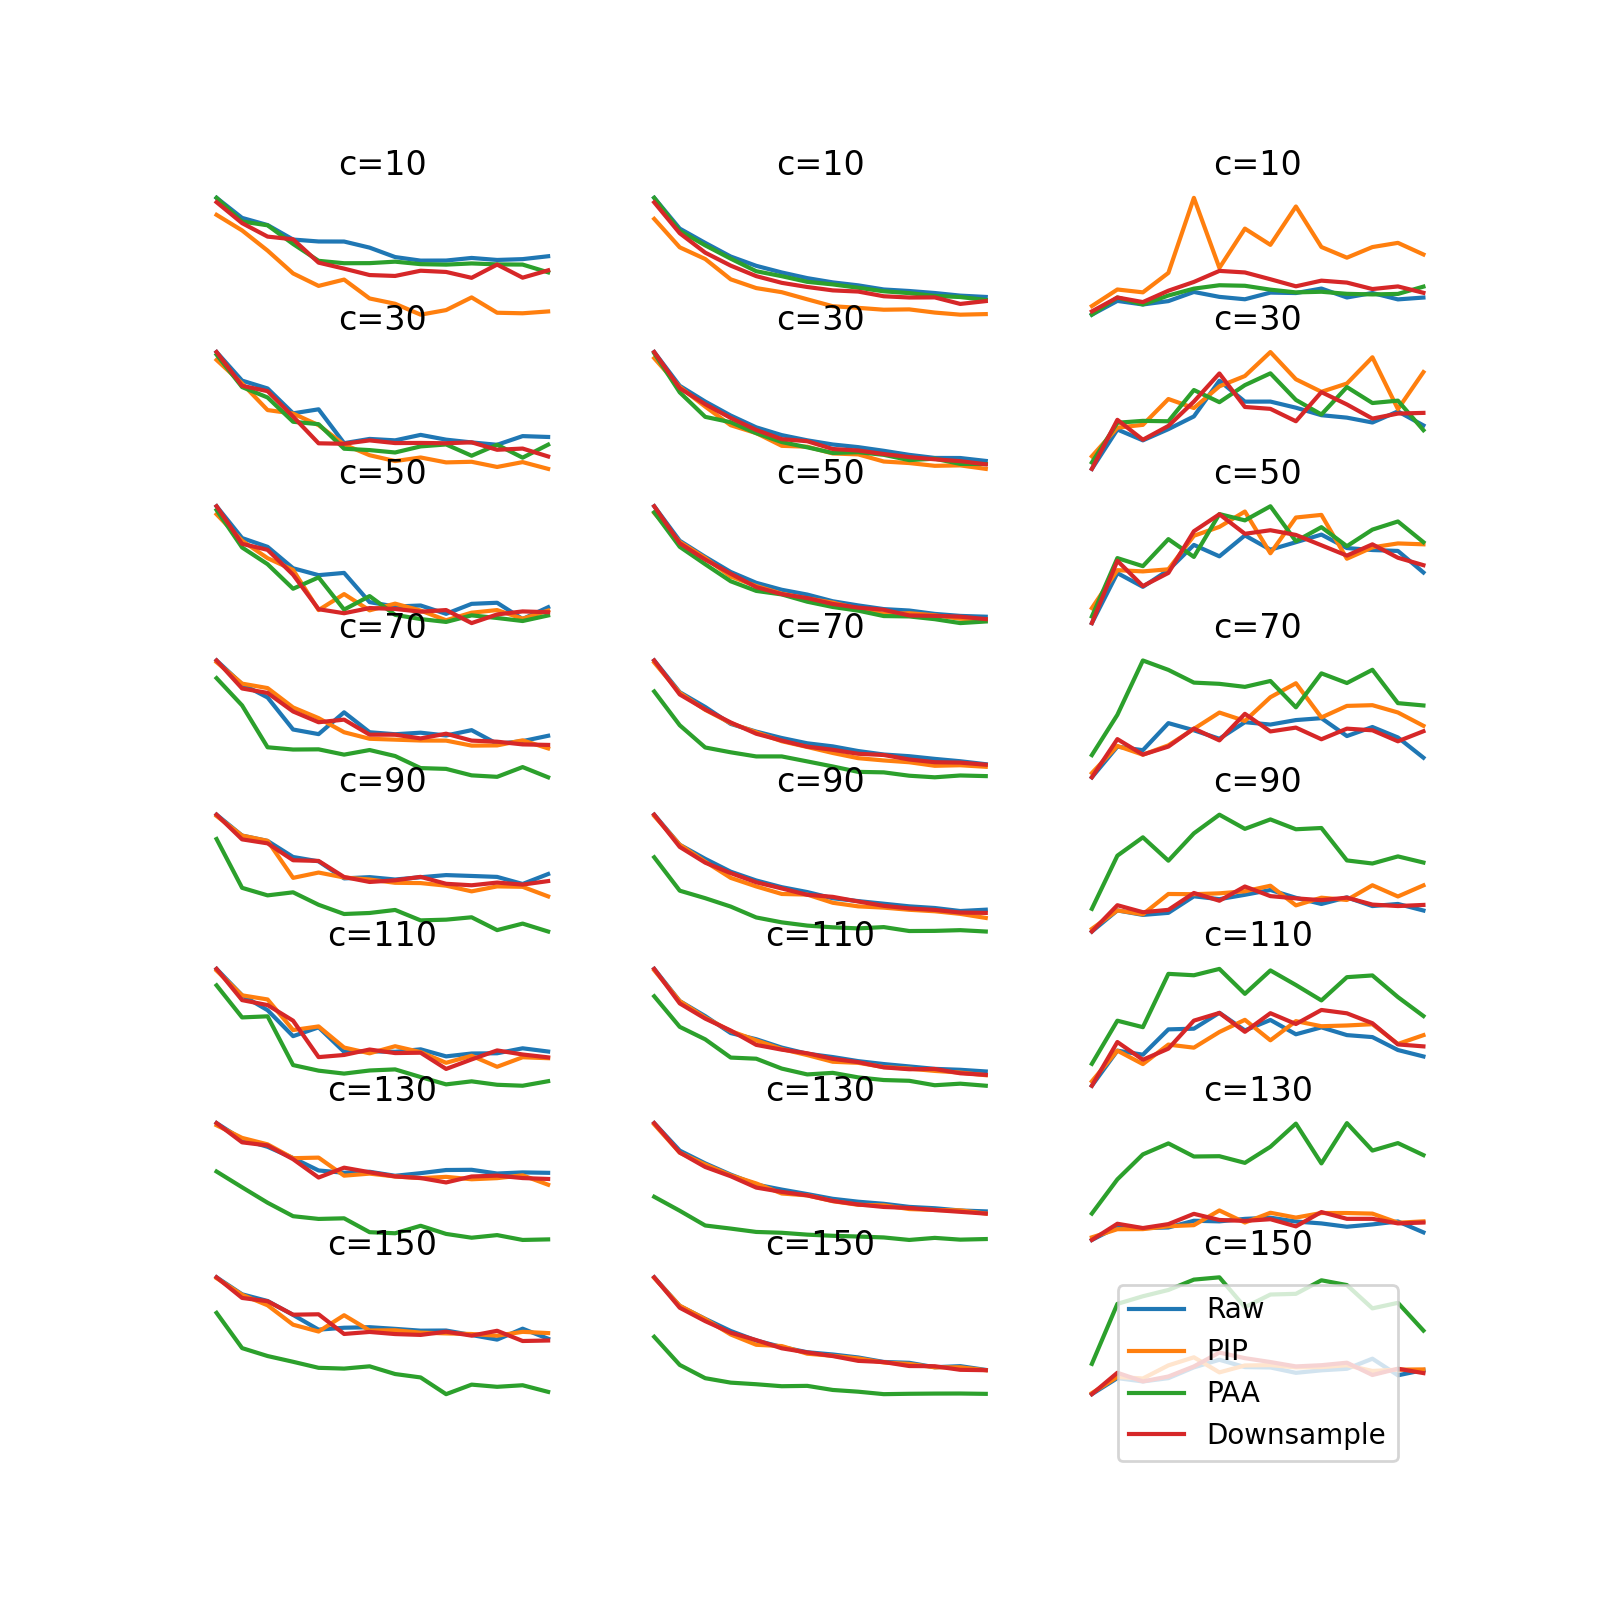
\includegraphics[width=0.3\columnwidth]{pippaac.png} 
    } 
    \subfigure[2012] { \label{fig:comparison2012} 
    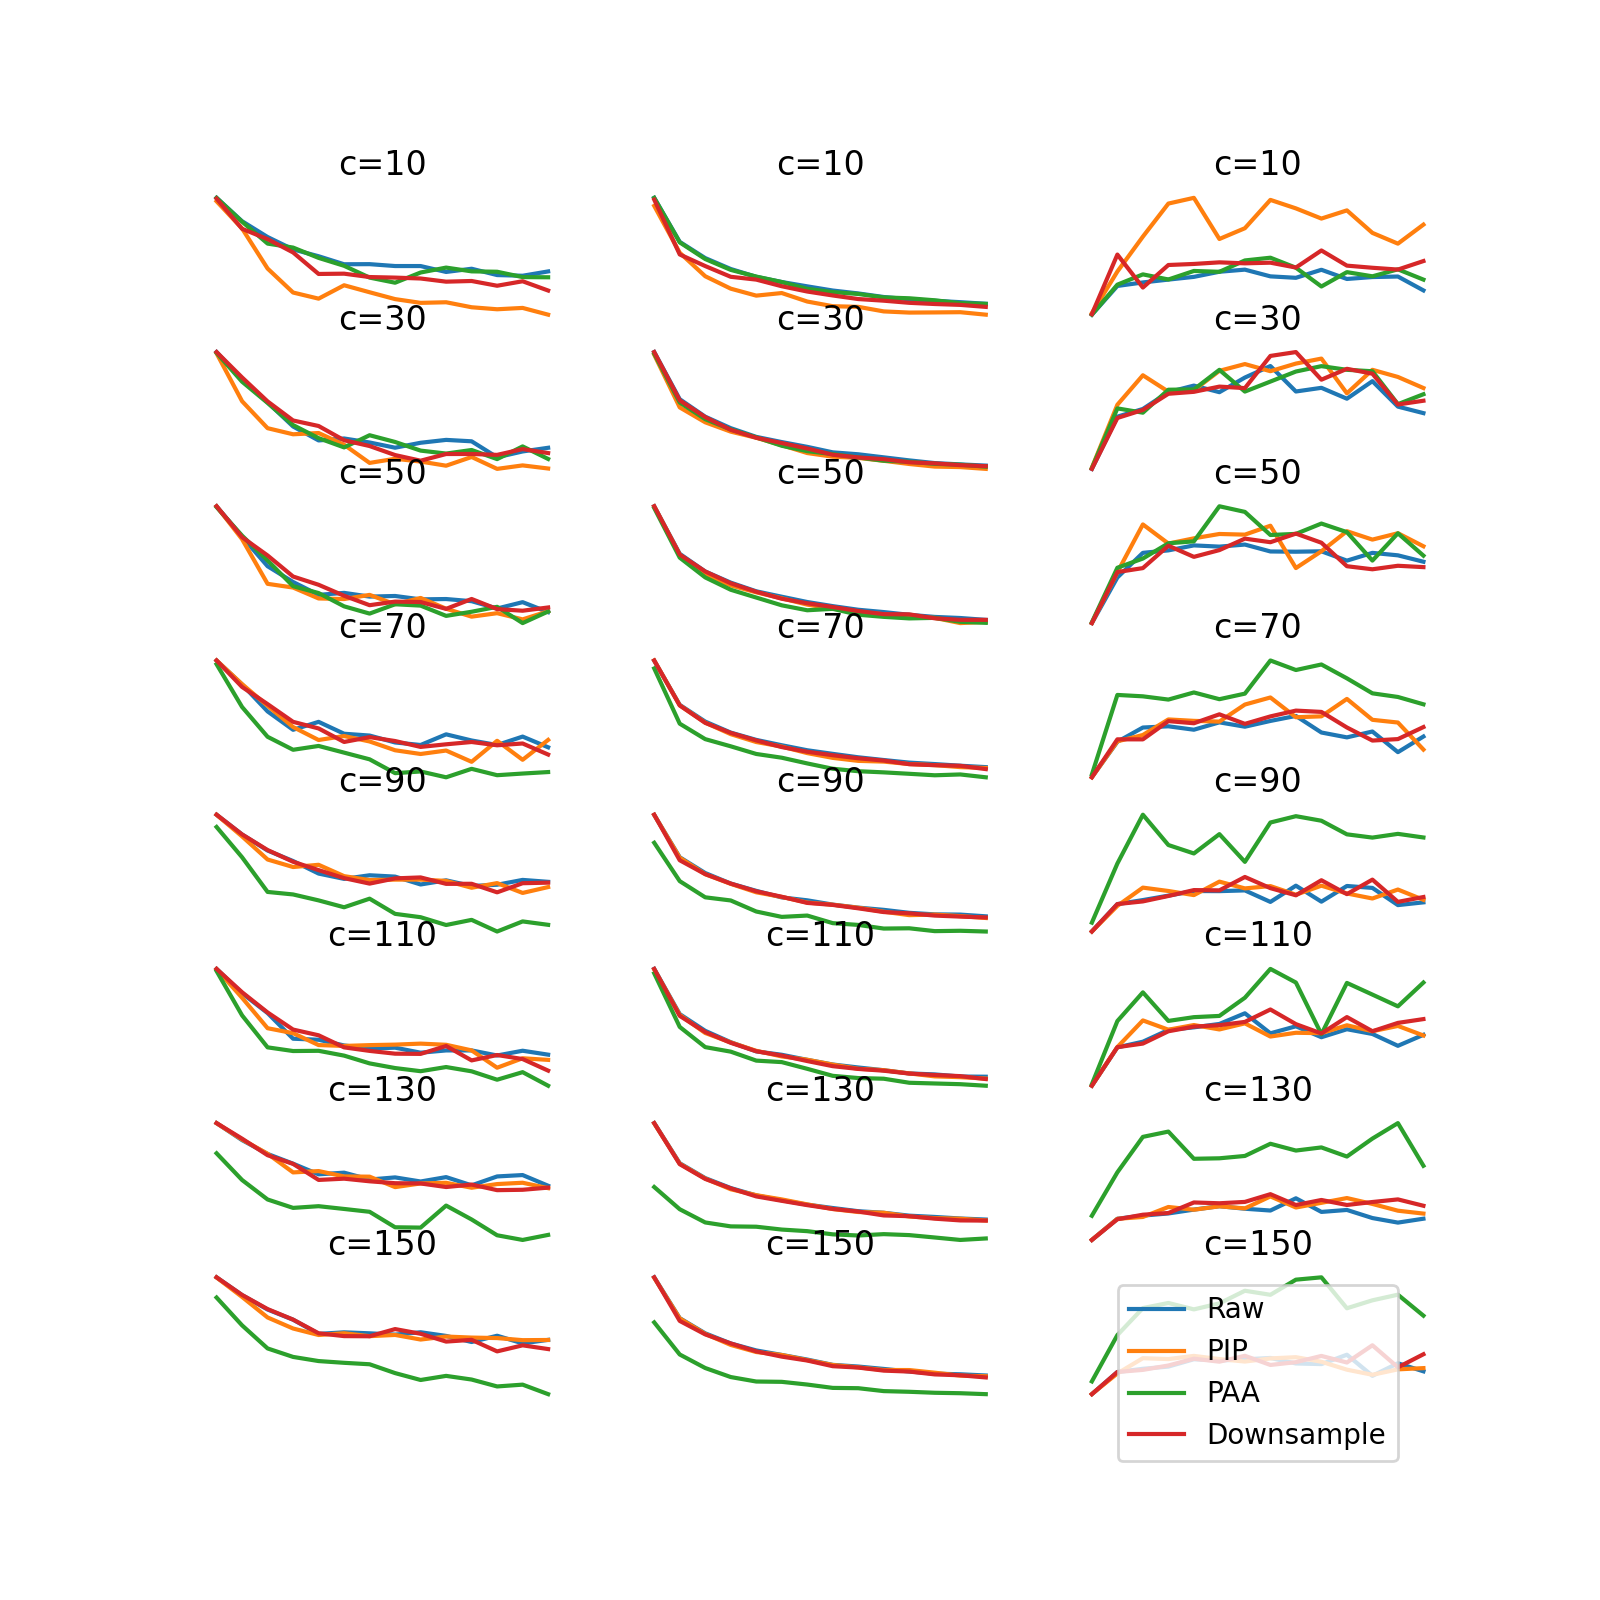
\includegraphics[width=0.3\columnwidth]{pippaac2012.png} 
    } 
    \subfigure[2013] { \label{fig:comparison2013} 
    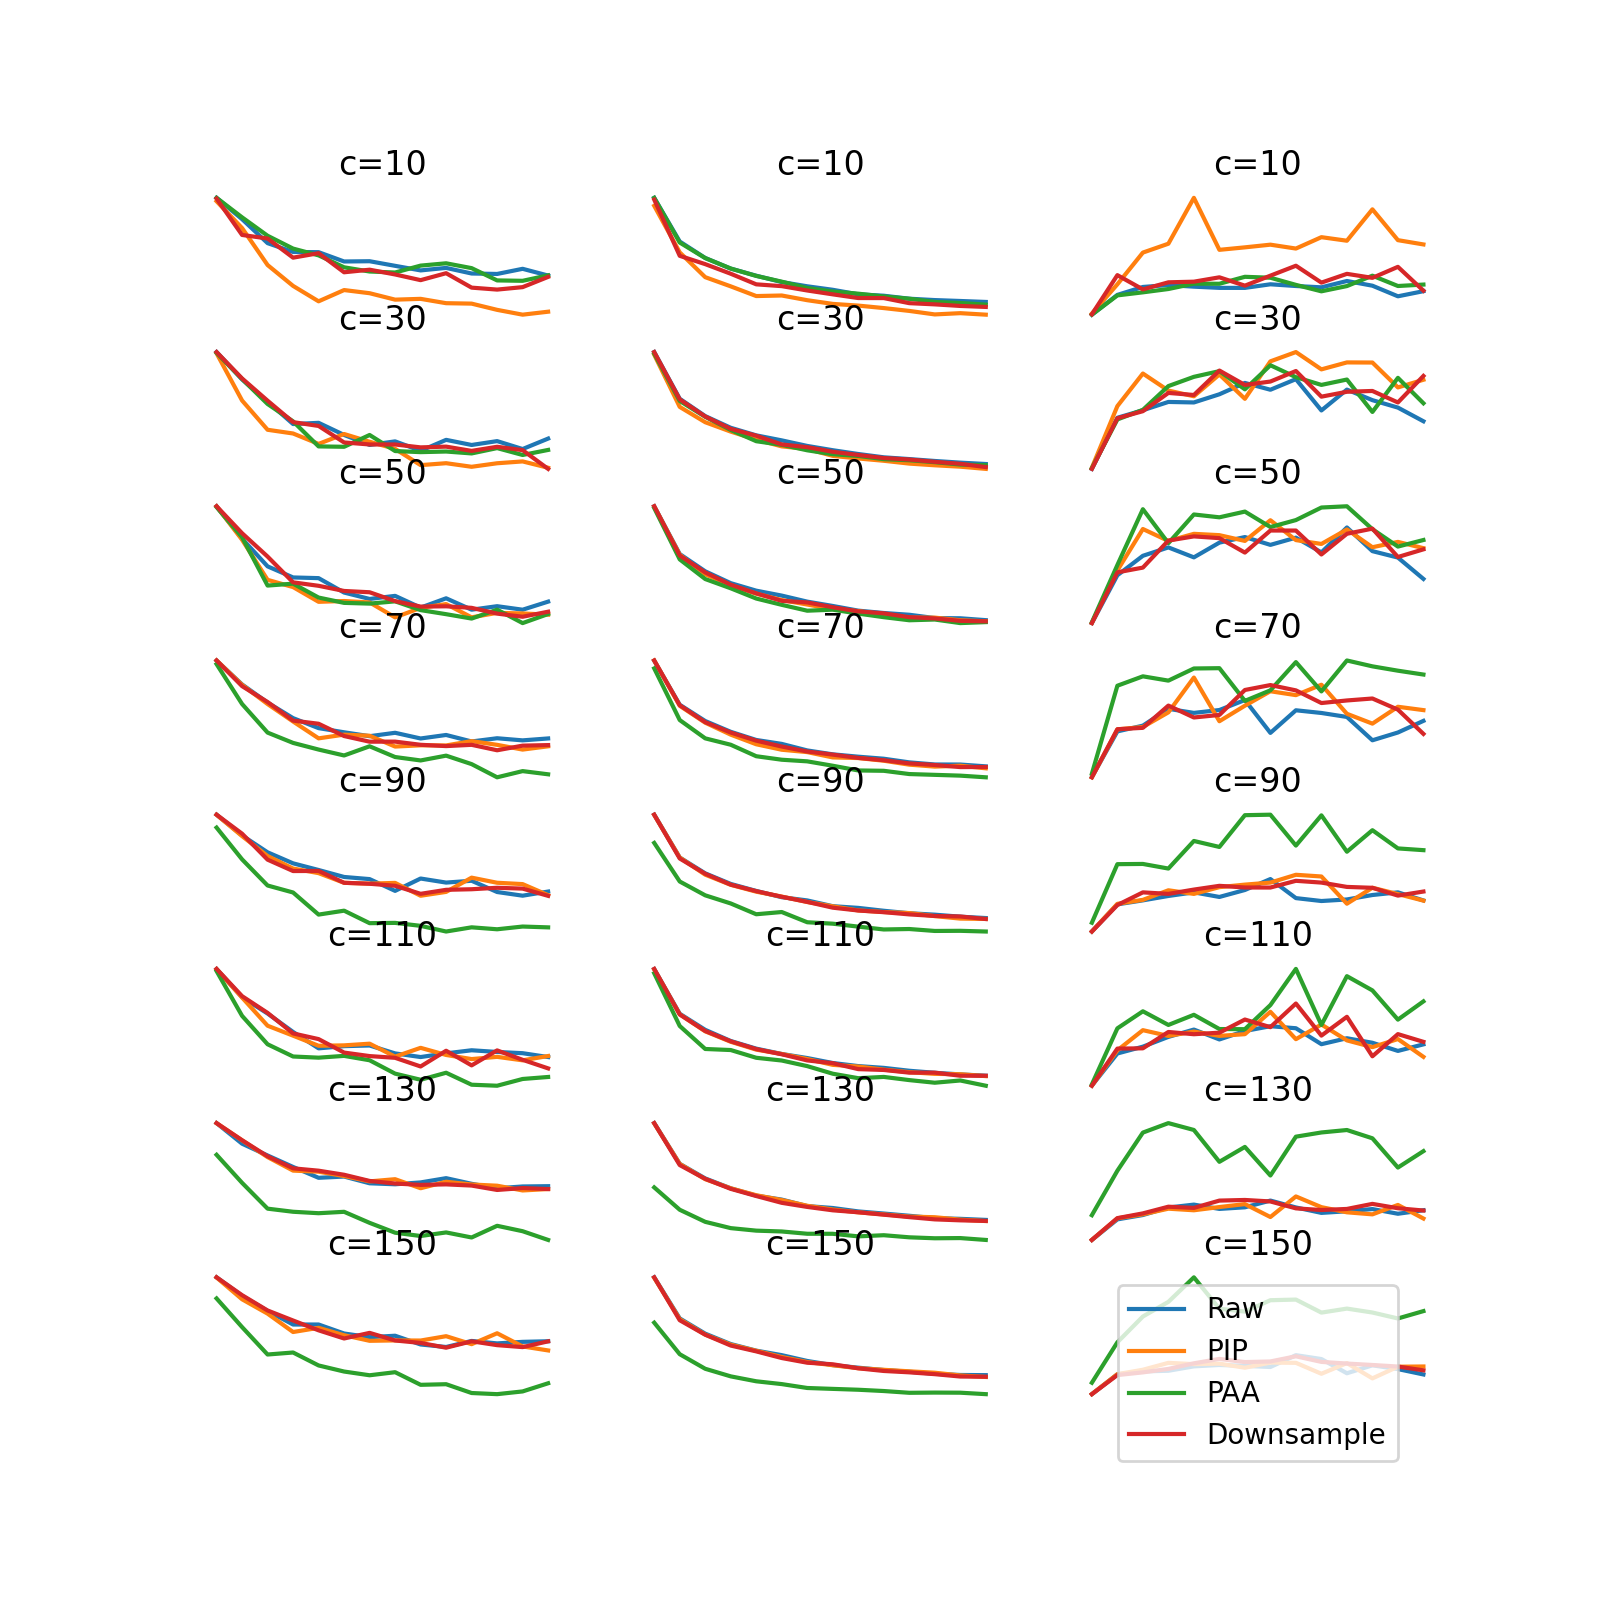
\includegraphics[width=0.3\columnwidth]{pippaac2013.png} 
    }
    \subfigure[2014] { \label{fig:comparison2014} 
    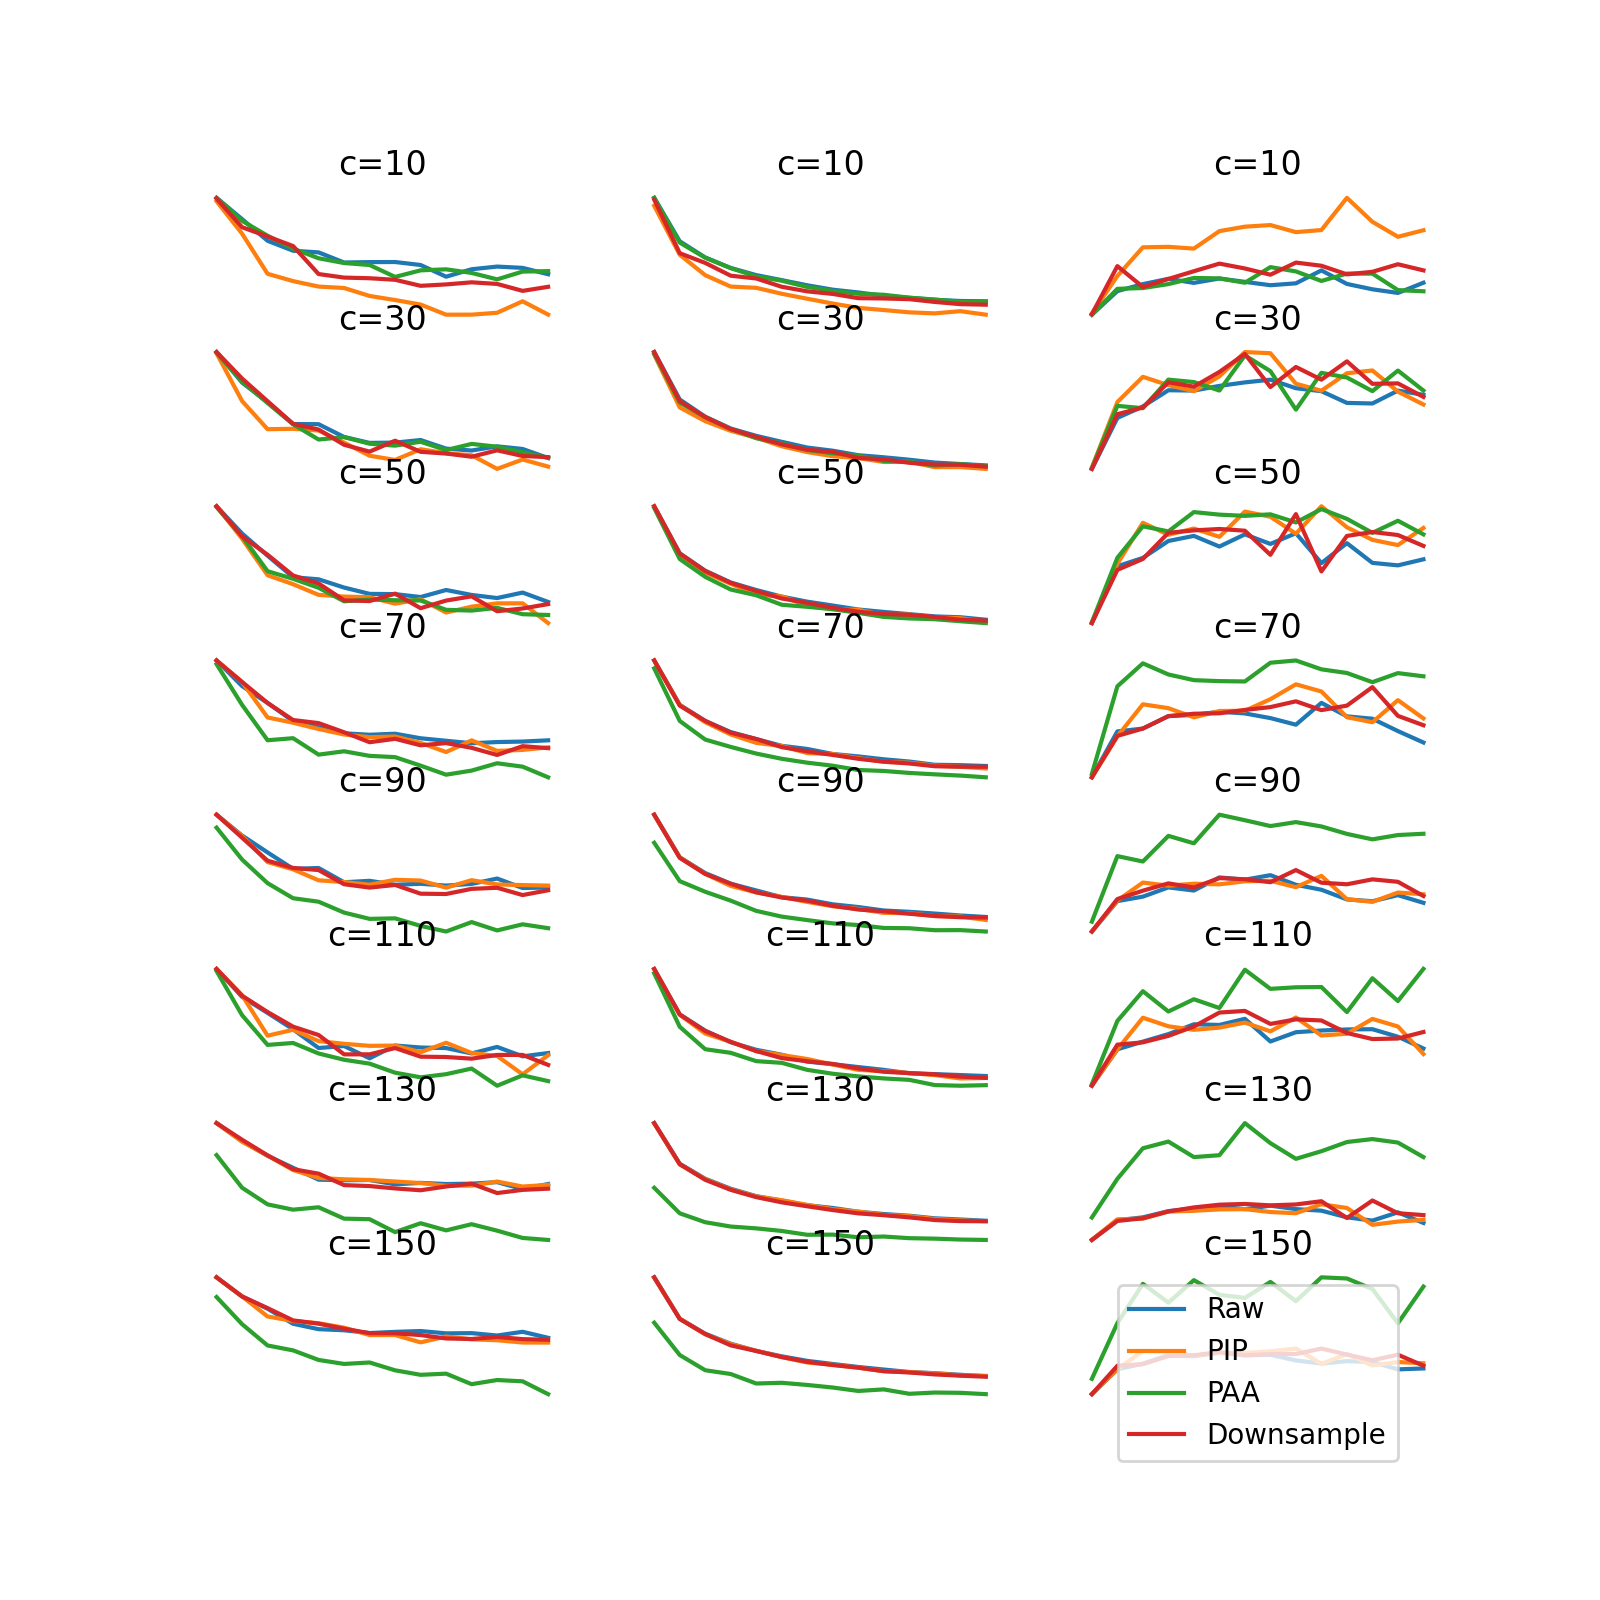
\includegraphics[width=0.3\columnwidth]{pippaac2014.png} 
    }
    \subfigure[2015] { \label{fig:comparison2015} 
    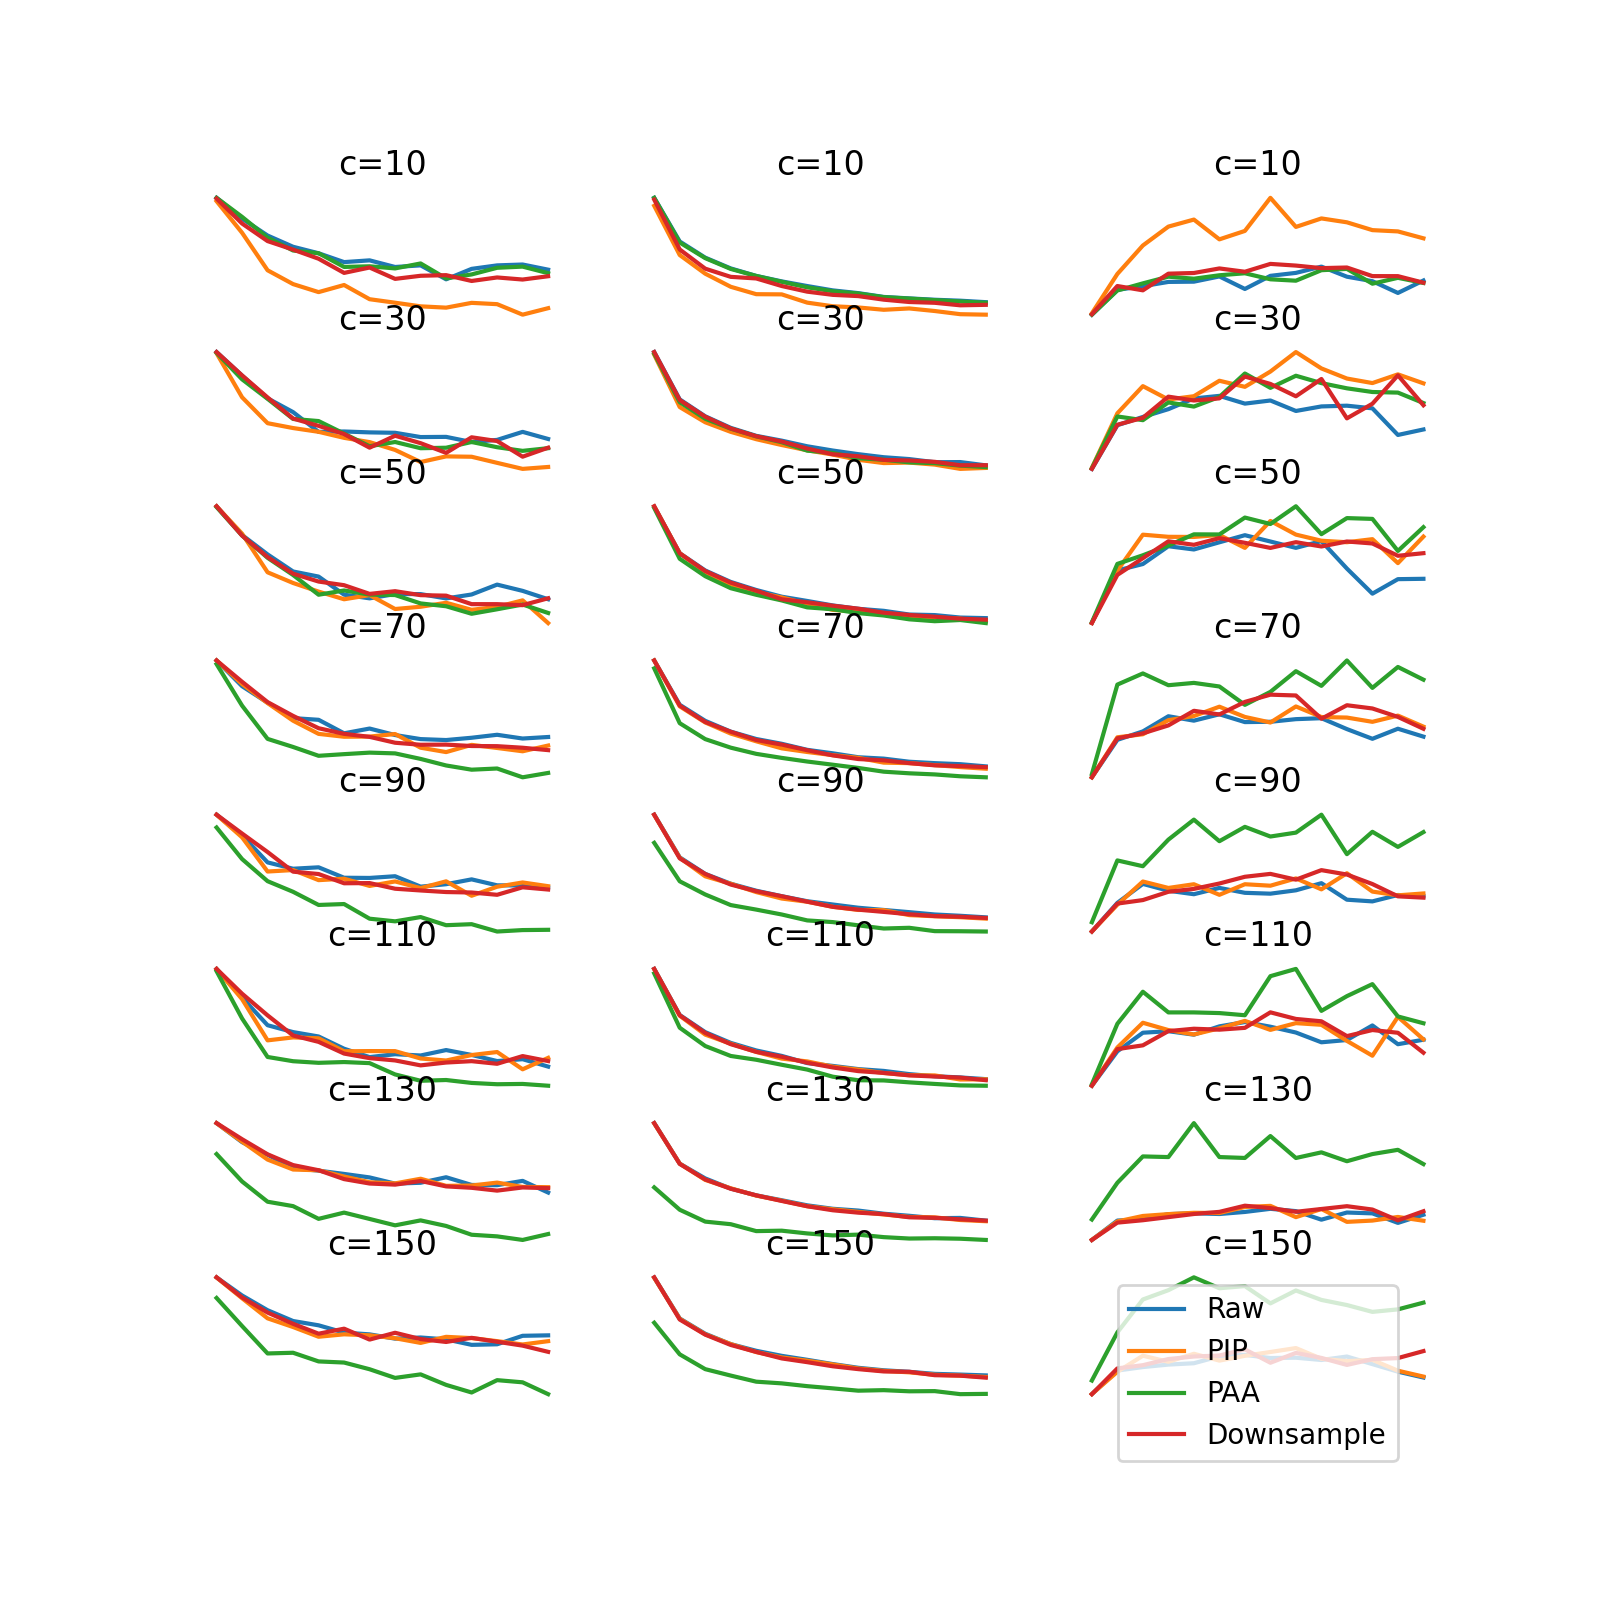
\includegraphics[width=0.3\columnwidth]{pippaac2015.png} 
    }
    \caption{ Different sequence length} 
    \label{fig:comparison1} 
\end{figure} 
\begin{figure}[!htbp]
    \centering 
    \subfigure[Raw 2011 (c=50)] { \label{fig:raw20111} 
    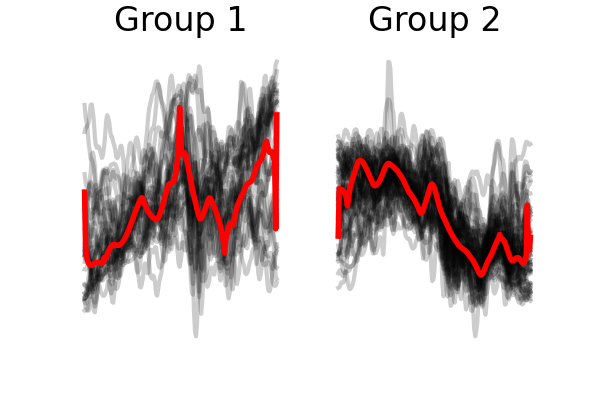
\includegraphics[width=0.4\columnwidth]{KshapeRaw1.png} 
    } 
    \subfigure[PIP 2011 (c=50)] { \label{fig:pip20111} 
    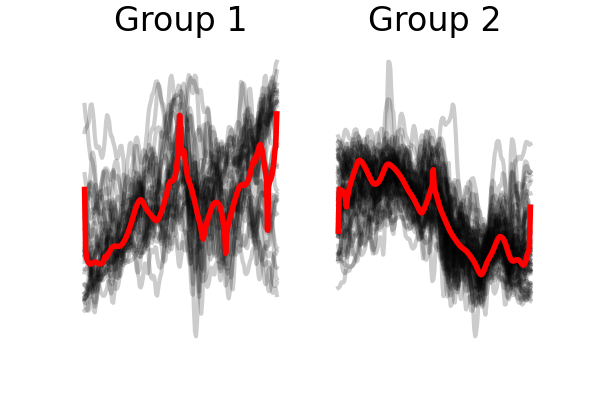
\includegraphics[width=0.4\columnwidth]{KshapePIP1.png} 
    }
    \subfigure[PAA 2011 (c=50)] { \label{fig:paa20111} 
    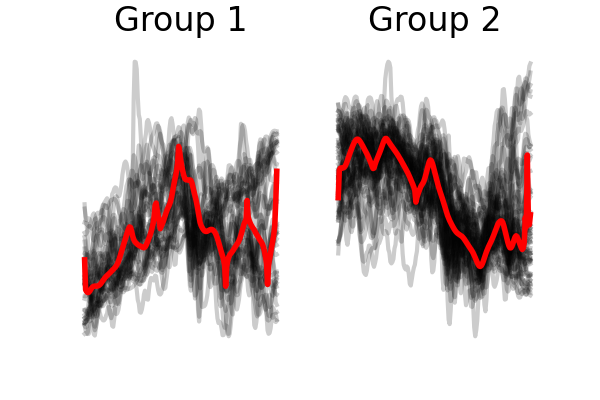
\includegraphics[width=0.4\columnwidth]{KshapePAA1.png} 
    }
    \subfigure[Downsampling 2011 (c=50)] { \label{fig:down20111} 
    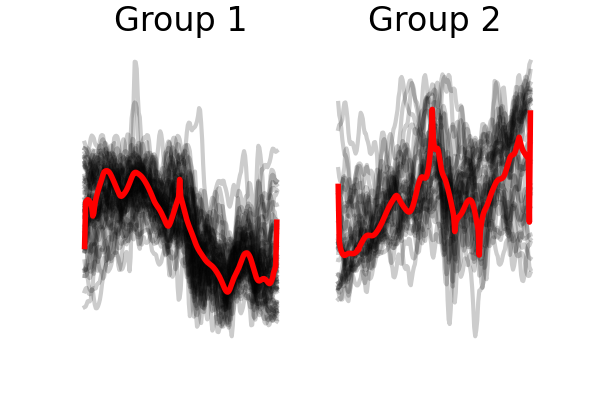
\includegraphics[width=0.4\columnwidth]{KShapedown1.png} 
    } 
    \caption{ Visual comparison } 
    \label{fig:pippaavisul} 
\end{figure} 
\\From those observations, it can be conclude that there is no improvement of using compression in terms of these three indexes. However, take the execution time and the storage cost into consideration, the compressed version is at least linearly faster than original version while use less memory, which emphasizes the importance of compression in time-series clustering tasks. 